\documentclass[norsk]{beamer}
\usepackage[utf8]{inputenc}
\usepackage[T1]{fontenc}
\usepackage{babel,textcomp}

\usetheme{Xal}

\begin{document}
\begin{frame}{Forsidetittel}
  Undertittel
\end{frame}

\begin{frame}{Lars Andreas Dal}
  \begin{columns}
    \column{.3\textwidth}
  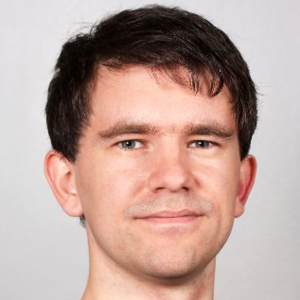
\includegraphics[width=\textwidth]{../people/lars.png}
    \column{.7\textwidth}
     \tiny
I am a physicist and software developer, and attained my Ph.D. in astroparticle physics at the University of Oslo in 2015. My Ph.D. work has involved large amounts of numerical simulations and software development, including parallelized programming and use of supercomputers. From my background in theoretical physics, I have excellent analytical skills, and I can quickly adapt to new problems.

My main fields of expertise are physics, scientific computing, mathematics, and programming. My primary programming expertise lies in C/C++ and Python, but I am also adept with a number of other programming languages, and can quickly pick up new ones. I am also very interested in game development and computer graphics, and have gained experience and much knowledge of these fields through personal hobby projects.
  \end{columns}
\end{frame}

\begin{frame}{Jonathan Feinberg}
  \begin{columns}
    \column{.3\textwidth}
  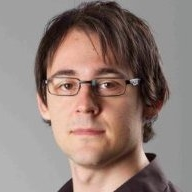
\includegraphics[width=\textwidth]{../people/jonathan.jpg}
    \column{.7\textwidth}
     \tiny
I hold a Ph.D. in mathematics at the University of Oslo with focus on statistics, probability and uncertainty quantification. My research interest include anything related to Bayesian theory, geo-statistics, graphical information system, machine learning, and language parsing.

I have much experience as a software developer from Simula Research Laboratory, Norway's highest ranked ICT research institution,  My programming skills include most things related to the Python programming language, which I have written a few software packages for. I am also familiar with other languages, like C++, Matlab and R, and can easily adapt beyond this.

I also have extensive experience as a teacher from institution as University of Oslo, Smerud Medical Research and House of Math.
  \end{columns}
\end{frame}

\begin{frame}{Eirik Gjerløw}
  \begin{columns}
    \column{.3\textwidth}
  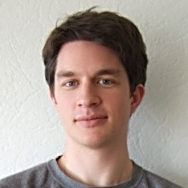
\includegraphics[width=\textwidth]{../people/eirik.png}
    \column{.7\textwidth}
     \tiny
I hold a Ph.D. in theoretical astrophysics from the University of Oslo, and my thesis revolved around numerical programming,  Bayesian data analysis, and signal processing. With a background in physics and mathematics, solving analytical problems is something I both enjoy and do well.

Much of my programming experience was obtained during my work with the European Space Agency (ESA), both during my thesis and later as a consultant. My specialties are numerical programming in the Python and Fortran programming languages, in which I have written
numerous libraries and programs for use in data analysis, with some experience also from C/C++ and MATLAB. I also have web programming and database experience, having worked with PHP/SQL for website development.

I have been teaching at both the Norwegian University of Science and Technology (NTNU) and the University of Oslo,  and have worked as a teacher for individuals as well as for large groups.
  \end{columns}
\end{frame}

\end{document}
